\documentclass[12pt,a4paper]{article}
\usepackage[utf8]{vietnam}
\usepackage{amsmath,amssymb}
\usepackage{geometry}
\geometry{top=1.5cm,bottom=1.2cm,left=1.4cm,right=1.4cm,headheight=28pt,headsep=12pt,footskip=18pt}
\usepackage{tikz}
\usepackage{xcolor}
\usepackage{enumerate}
\usepackage{graphicx}
\usepackage[version=4]{mhchem}
\usepackage{fancyhdr}
\usepackage{ex_test}

\renewcommand{\baselinestretch}{0.96}
\setlength{\parskip}{0pt}

\definecolor{hfRed}{RGB}{211,47,47}
\definecolor{hfGreen}{RGB}{139,195,144}

\pagestyle{fancy}
\fancyhf{}
\fancyhead[L]{\small\itshape\color{hfRed} Tài liệu lưu hành nội bộ}
\fancyhead[R]{\small\itshape\color{hfRed} Thầy \textbf{TRẦN VĂN THẠNH} - 0777.470.803}
\renewcommand{\headrulewidth}{0.8pt}
\renewcommand{\headrule}{\hbox to\headwidth{\color{hfGreen}\leaders\hrule height \headrulewidth\hfill}}

\fancyfoot[L]{\small\itshape\color{hfRed} CS1: 6/15 Nguyễn Hoàng, P. Kim Long, TP Huế \quad|\quad CS2: 24 Đặng Thái Thân, TP Huế}
\fancyfoot[R]{\small\bfseries\color{hfRed} Trang \thepage}
\renewcommand{\footrulewidth}{0.8pt}
\renewcommand{\footrule}{\hbox to\headwidth{\color{hfGreen}\leaders\hrule height \footrulewidth\hfill}}

\fancypagestyle{firstpage}{
  \fancyhf{}
  \renewcommand{\headrulewidth}{0pt}
  \fancyfoot[L]{\small\itshape\color{hfRed} CS1: 6/15 Nguyễn Hoàng, P. Kim Long, TP Huế \quad|\quad CS2: 24 Đặng Thái Thân, TP Huế}
  \fancyfoot[R]{\small\bfseries\color{hfRed} Trang \thepage}
  \renewcommand{\footrulewidth}{0.8pt}
  \renewcommand{\footrule}{\hbox to\headwidth{\color{hfGreen}\leaders\hrule height \footrulewidth\hfill}}
}

\begin{document}
\thispagestyle{firstpage}

\noindent
\begin{minipage}[t]{0.44\textwidth}
	\centering\fontsize{10pt}{12pt}\selectfont
	\textbf{SỞ GIÁO DỤC VÀ ĐÀO TẠO THỪA THIÊN HUẾ}\\
	\textbf{ĐỀ CHÍNH THỨC}\\
	\textit{(Đề thi có 04 trang)}
\end{minipage}\hfill
\begin{minipage}[t]{0.54\textwidth}
	\centering\fontsize{10.5pt}{13pt}\selectfont
	\textbf{ĐỀ KIỂM TRA ĐỊNH KỲ CHƯƠNG 4 (HYDROCARBON)}\\
	\textbf{MÔN: HOÁ HỌC - LỚP 11}\\
	\textit{Thời gian làm bài: 45 phút, không kể thời gian phát đề}
	
	\smallskip
	\fbox{\textbf{MÃ ĐỀ: 110}}
\end{minipage}

\smallskip
\noindent\hrulefill
\smallskip

\noindent\textbf{Họ, tên thí sinh:} \dotfill\ \textbf{Lớp:} \dotfill\ \textbf{Số báo danh:} \dotfill

\smallskip
\noindent\textit{(Cho biết nguyên tử khối: H = 1; C = 12; N = 14; O = 16; F = 19; Na = 23; Mg = 24; Al = 27; P = 31; S = 32; Cl = 35,5; K = 39; Ca = 40; Fe = 56; Cu = 64; Br = 80; Ag = 108; Ba = 137).}
\smallskip

\noindent\textbf{\large PHẦN I. Câu trắc nghiệm nhiều phương án lựa chọn.}
\textit{Thí sinh trả lời từ câu 1 đến câu 18. Mỗi câu hỏi thí sinh chỉ chọn một phương án.}
\vspace{0.2cm}

\Opensolutionfile{ans}[ans-hoa11-de10hs]

\begin{ex}
Chất nào sau đây là pentane?
\choice
{$\ce{CH4}$}
{\True $\ce{CH3[CH2]3CH3}$}
{$\ce{CH3[CH2]2CH3}$}
{$\ce{CH3CH2CH3}$}
\loigiai{
Pentane là alkane no, mạch hở chứa 5 nguyên tử carbon ($\ce{C5H12}$), có công thức cấu tạo thu gọn là $\ce{CH3[CH2]3CH3}$ (hay $\ce{CH3-CH2-CH2-CH2-CH3}$).
}
\end{ex}

\begin{ex}
Phát biểu nào sau đây \textbf{không đúng} khi nói về tính chất vật lý của alkane?
\choice
{Các alkane đều nhẹ hơn nước}
{Các alkane không tan trong nước}
{Ở điều kiện thường, các alkane từ $\ce{C1}$ đến $\ce{C4}$ ở thể khí, từ $\ce{C5}$ đến khoảng $\ce{C17}$ ở thể lỏng, từ khoảng $\ce{C18}$ trở lên ở thể rắn}
{\True Các alkane không tan hoặc tan rất ít trong các dung môi hữu cơ}
\loigiai{
Alkane là những phân tử không phân cực hoặc phân cực rất yếu nên tan tốt trong các dung môi hữu cơ không phân cực (như ether, benzene, chloroform,...), do đó phát biểu ``không tan hoặc tan rất ít trong các dung môi hữu cơ'' là sai.
}
\end{ex}

\begin{ex}
Độ dài liên kết bội giữa hai nguyên tử carbon luôn \dots độ dài liên kết đơn giữa hai nguyên tử carbon đó. Cụm từ thích hợp điền vào chỗ trống là
\choice
{\True ngắn hơn}
{dài hơn}
{bằng nhau}
{gấp đôi}
\loigiai{
Do liên kết bội (gồm liên kết $\sigma$ và liên kết $\pi$) có mật độ electron giữa hai hạt nhân carbon lớn hơn, lực hút giữa hai hạt nhân mạnh hơn kéo hai nguyên tử carbon lại gần nhau hơn nên độ dài liên kết bội ngắn hơn độ dài liên kết đơn giữa hai nguyên tử carbon.
}
\end{ex}

\begin{ex}
Thành phần chính của khí biogas là
\choice
{ethane}
{propane}
{\True methane}
{butane}
\loigiai{
Methane ($\ce{CH4}$) chiếm khoảng 50 -- 70\% thể tích của khí sinh học (biogas), sinh ra từ sự phân hủy kị khí chất thải hữu cơ.
}
\end{ex}

\begin{ex}
Alkene, alkyne là những hydrocarbon không no, mạch hở, trong phân tử có chứa
\choice
{liên kết $\pi$}
{liên kết đơn}
{\True liên kết bội}
{vòng benzene}
\loigiai{
Alkene chứa 1 liên kết đôi $\ce{C=C}$, alkyne chứa 1 liên kết ba $\ce{C#C}$. Các liên kết đôi và liên kết ba này được gọi chung là liên kết bội.
}
\end{ex}

\begin{ex}
Bảng dưới đây thể hiện nhiệt độ sôi của một số chất:
\begin{itemize}
    \setlength\itemsep{0pt}
    \item Ethene (chất Y): nhiệt độ sôi là $-103{,}7$~$^\circ\text{C}$
    \item Propene (chất X): nhiệt độ sôi là $-47{,}7$~$^\circ\text{C}$
    \item But-1-ene (chất Z): nhiệt độ sôi là $-6{,}3$~$^\circ\text{C}$
    \item Pent-1-ene (chất T): nhiệt độ sôi là $30$~$^\circ\text{C}$
\end{itemize}
Ở điều kiện thường ($25$~$^\circ\text{C}$), chất tồn tại ở trạng thái lỏng là
\choice
{Y}
{Z}
{X}
{\True T}
\loigiai{
Ở điều kiện thường ($25$~$^\circ\text{C}$), chất T (pent-1-ene) có nhiệt độ sôi là $30$~$^\circ\text{C} > 25$~$^\circ\text{C}$ nên tồn tại ở thể lỏng. Các chất còn lại có nhiệt độ sôi thấp hơn $25$~$^\circ\text{C}$ nên ở thể khí.
}
\end{ex}

\begin{ex}
Chất nào sau đây làm mất màu dung dịch bromine ở điều kiện thường?
\choice
{Butane}
{\True But-1-ene}
{Isobutane}
{Propane}
\loigiai{
But-1-ene là alkene có liên kết đôi $\ce{C=C}$ nên tham gia phản ứng cộng làm mất màu dung dịch nước bromine:
\[\ce{CH2=CH-CH2-CH3 + Br2 -> CH2Br-CHBr-CH2-CH3}\]
}
\end{ex}

\begin{ex}
Khi cho carbide kim loại tác dụng với nước thì carbide kim loại nào sau đây \textbf{không thể} tạo ra acetylene ($\ce{C2H2}$)?
\choice
{$\ce{CaC2}$}
{$\ce{Mg2C3}$}
{\True $\ce{Al4C3}$}
{$\ce{Na2C2}$}
\loigiai{
Nhôm carbide tác dụng với nước tạo thành methane, không tạo ra acetylene:
\[\ce{Al4C3 + 12H2O -> 4Al(OH)3 + 3CH4 ^}\]
Trong khi đó, $\ce{CaC2 + 2H2O -> Ca(OH)2 + C2H2 ^}$.
}
\end{ex}

\begin{ex}
Chất nào sau đây thuộc dãy đồng đẳng của benzene?
\choice
{$\ce{C6H5CH=CH2}$}
{$\ce{C10H8}$}
{$\ce{C6H5-C6H5}$}
{\True $\ce{C8H10}$}
\loigiai{
Dãy đồng đẳng của benzene (alkylbenzene) có công thức chung $\ce{C_nH_{2n-6}}$ ($n \ge 6$). Với $n = 8 \implies \ce{C8H10}$ (ethylbenzene hoặc dimethylbenzene).
}
\end{ex}

\begin{ex}
Cho các hydrocarbon sau: benzene, toluene, naphthalene, ethylene, acetylene, methane. Số chất ở thể lỏng ở điều kiện thường là
\choice
{1}
{\True 2}
{3}
{4}
\loigiai{
Ở điều kiện thường:
- Thể khí: methane, ethylene, acetylene.
- Thể lỏng: benzene, toluene.
- Thể rắn: naphthalene.
Vậy có 2 chất ở thể lỏng.
}
\end{ex}

\begin{ex}
(SBT - KNTT). Nitro hoá benzene bằng hỗn hợp $\ce{HNO3}$ đặc và $\ce{H2SO4}$ đặc ở nhiệt độ $\le 50$~$^\circ\text{C}$, tạo thành chất hữu cơ X. Phát biểu nào sau đây về X \textbf{không đúng}?
\choice
{Tên của X là nitrobenzene}
{X là chất lỏng, sánh như dầu}
{X có màu vàng}
{\True X tan tốt trong nước}
\loigiai{
Nitrobenzene ($\ce{C6H5NO2}$) là chất lỏng sánh màu vàng nhạt, hầu như không tan trong nước và nặng hơn nước chìm xuống đáy. Do đó phát biểu ``X tan tốt trong nước'' là sai.
}
\end{ex}

\begin{ex}
(SBT - CD). Nhỏ 1 mL nước bromine vào ống nghiệm đựng 1 mL hexane, chiếu sáng và lắc đều. Hiện tượng quan sát được là
\choice
{trong ống nghiệm có chất lỏng đồng nhất}
{\True màu của nước bromine bị mất}
{màu của bromine không thay đổi}
{trong ống nghiệm xuất hiện kết tủa}
\loigiai{
Dưới tác dụng của ánh sáng, hexane tham gia phản ứng thế halogen với bromine làm tiêu hao $\ce{Br2}$: $\ce{C6H14 + Br2 ->[as] C6H13Br + HBr}$, nên màu vàng cam của nước bromine bị mất.
}
\end{ex}

\begin{ex}
(SBT - KNTT). Arene hay còn gọi là hydrocarbon thơm là những hydrocarbon trong phân tử có chứa một hay nhiều
\choice
{\True vòng benzene}
{liên kết đơn}
{liên kết đôi}
{liên kết ba}
\loigiai{
Hydrocarbon thơm (arene) là những hydrocarbon trong phân tử có chứa một hay nhiều vòng benzene.
}
\end{ex}

\begin{ex}
(SBT - CTST). Cho alkane có công thức cấu tạo:
\begin{center}
    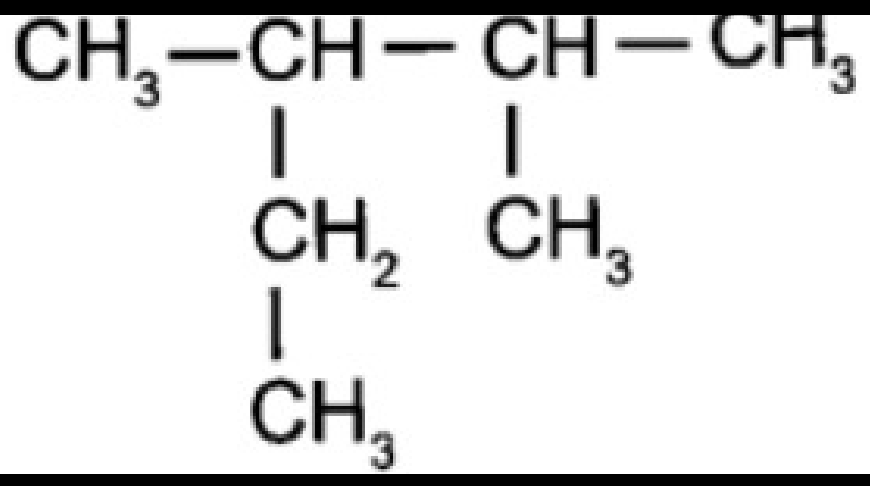
\includegraphics[width=3.5cm]{images_crop_hoa11_de10/hoa11_de10_cau14_alkane.png}
\end{center}
Danh pháp thay thế của alkane trên là
\choice
{2-ethyl-3-methylbutane}
{2-methyl-3-ethylbutane}
{3,4-dimethylpentane}
{\True 2,3-dimethylpentane}
\loigiai{
Mạch chính dài nhất chứa 5 nguyên tử carbon (pentane). Đánh số mạch carbon từ đầu gần nhánh hơn:
$\ce{C^5H3-C^4H2-C^3H(CH3)-C^2H(CH3)-C^1H3}$.
Tại vị trí C-2 và C-3 có hai nhóm methyl ($\ce{-CH3}$). Tên thay thế là 2,3-dimethylpentane.
}
\end{ex}

\begin{ex}
(SBT - CD). Cho pent-2-ene phản ứng với dung dịch $\ce{KMnO4}$ ở nhiệt độ phòng có thể thu được sản phẩm hữu cơ có công thức cấu tạo nào sau đây?
\choice
{\True $\ce{CH3CH2CH(OH)CH(OH)CH3}$}
{$\ce{CH3CH2CH2CH(OH)CH3}$}
{$\ce{CH3CH(OH)CH2CH(OH)CH3}$}
{$\ce{CH3CH2CH(OH)CH2CH3}$}
\loigiai{
Phản ứng oxi hóa không hoàn toàn alkene bằng dung dịch $\ce{KMnO4}$ ở điều kiện thường tạo diol liền kề:
\[\ce{3CH3-CH=CH-CH2-CH3 + 2KMnO4 + 4H2O -> 3CH3-CH(OH)-CH(OH)-CH2-CH3 + 2MnO2 v + 2KOH}\]
}
\end{ex}

\begin{ex}
Tính chất nào \textbf{không phải} của benzene?
\choice
{Tác dụng với $\ce{Br2}$ ($t^\circ$, Fe)}
{Tác dụng với $\ce{HNO3}$ (đ) / $\ce{H2SO4}$ (đ)}
{\True Tác dụng với dung dịch $\ce{KMnO4}$}
{Tác dụng với $\ce{Cl2}$ ($as$)}
\loigiai{
Hệ electron $\pi$ vòng thơm benzene rất bền vững nên không phản ứng và không làm mất màu dung dịch $\ce{KMnO4}$ kể cả khi đun nóng.
}
\end{ex}

\begin{ex}
(SBT - KNTT). Cho các hydrocarbon sau:
\begin{center}
    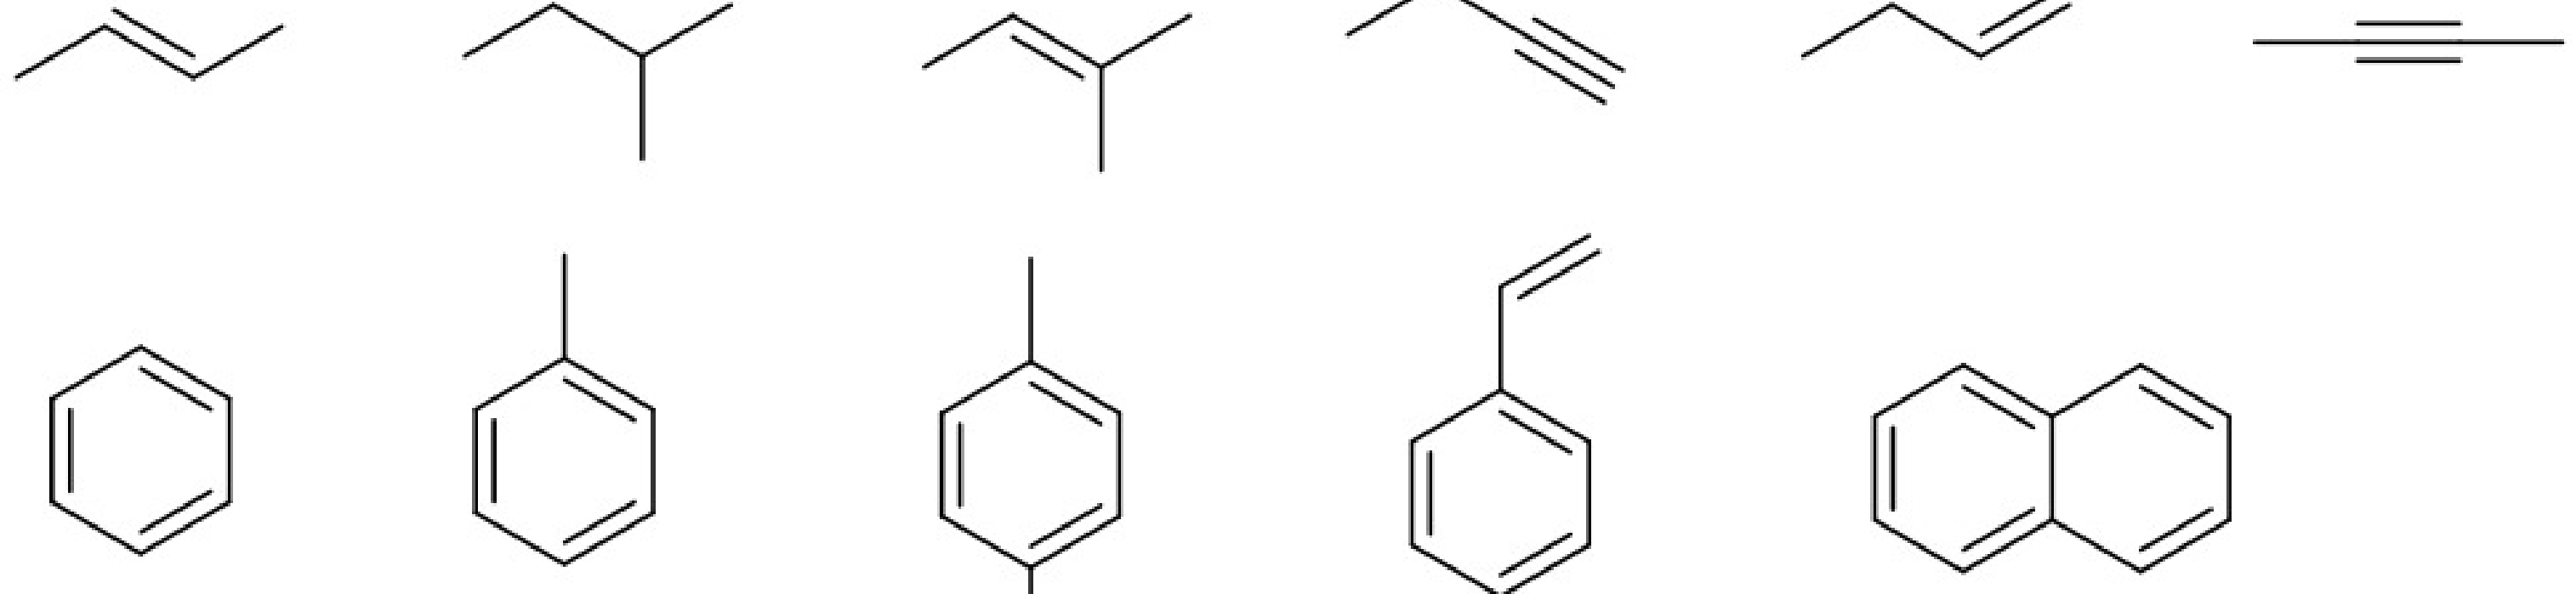
\includegraphics[width=11.5cm]{images_crop_hoa11_de10/hoa11_de10_cau17_hydrocarbons.png}
\end{center}
Một số nhận định về các hydrocarbon trên là:
\begin{enumerate}[(1)]
    \setlength\itemsep{0pt}
    \item Số phân tử hydrocarbon không no bằng 5;
    \item Số phân tử alkene bằng 3;
    \item Số phân tử alkyne bằng 2;
    \item Số phân tử thuộc dãy đồng đẳng của benzene bằng 3.
\end{enumerate}
Trong các nhận định này, số nhận định đúng bằng
\choice
{1}
{2}
{3}
{\True 4}
\loigiai{
Phân tích 11 chất:
- Hàng 1 (mạch hở): but-2-ene (alkene), 2-methylbutane (alkane no), 2-methylbut-2-ene (alkene), but-1-yne (alkyne), but-1-ene (alkene), but-2-yne (alkyne).
- Hàng 2 (vòng thơm): benzene, toluene, p-xylene (3 đồng đẳng của benzene); styrene; naphthalene.
Xét từng nhận định:
(1) Hydrocarbon không no gồm 5 chất: but-2-ene, 2-methylbut-2-ene, but-1-yne, but-1-ene, but-2-yne $\implies$ Đúng.
(2) Alkene gồm 3 chất: but-2-ene, 2-methylbut-2-ene, but-1-ene $\implies$ Đúng.
(3) Alkyne gồm 2 chất: but-1-yne, but-2-yne $\implies$ Đúng.
(4) Dãy đồng đẳng benzene gồm 3 chất: benzene, toluene, p-xylene $\implies$ Đúng.
Cả 4 nhận định đều đúng $\implies$ Chọn D.
}
\end{ex}

\begin{ex}
Benzene gây tác hại lên tủy xương và làm giảm lượng hồng cầu, dẫn đến thiếu máu. Benzene cũng có thể ảnh hưởng đến hệ thống miễn dịch, làm tăng nguy cơ nhiễm trùng. Khi hút mỗi điếu thuốc lá, người hút đưa vào cơ thể $50\ \mu\text{g}$ benzene. Nếu một người hút 15 điếu thuốc lá mỗi ngày thì lượng benzene người đó hấp thụ vào cơ thể là bao nhiêu g?
\choice
{$7{,}5 \cdot 10^{-5}$}
{$15 \cdot 10^{-5}$}
{\True $7{,}5 \cdot 10^{-4}$}
{$15 \cdot 10^{-4}$}
\loigiai{
Đổi $1\ \mu\text{g} = 10^{-6}\text{ g}$.
Lượng benzene hấp thụ mỗi ngày:
\[m = 15 \times 50\ \mu\text{g} = 750\ \mu\text{g} = 750 \times 10^{-6}\text{ g} = 7{,}5 \cdot 10^{-4}\text{ g}.\]
}
\end{ex}

\Closesolutionfile{ans}

\vspace{0.3cm}
\noindent\textbf{\large PHẦN II. Câu trắc nghiệm đúng sai.}
\textit{Thí sinh trả lời từ câu 1 đến câu 4. Trong mỗi ý a), b), c), d) ở mỗi câu, thí sinh chọn đúng hoặc sai.}
\vspace{0.2cm}

\begin{ex}
Dựa vào đặc điểm cấu tạo phân tử của các alkane thì:
\choiceTF
{\True Alkane là những hydrocarbon mạch hở chỉ chứa liên kết đơn trong phân tử nên được gọi là hydrocarbon bão hoà và có công thức chung $\ce{C_nH_{2n+2}}$ ($n \ge 1$)}
{Alkane là những hydrocarbon chỉ chứa liên kết đơn trong phân tử nên được gọi là hydrocarbon bão hoà và có công thức chung $\ce{C_nH_{2n+2}}$ ($n \ge 2$)}
{\True Phân tử của một alkane trong sáp nến có 52 nguyên tử hydrogen, thì số nguyên tử carbon trong phân tử alkane là 25}
{Cho hai chất: (1) $\ce{CH3-CH2-CH3}$ ; (2) $\ce{CH3-CH(CH3)-CH3}$. Alkane (1) là alkane có mạch phân nhánh}
\loigiai{
a) Đúng: Đây là định nghĩa và công thức phân tử chung chuẩn xác của alkane.\\
b) Sai: Điều kiện $n \ge 1$ ($\ce{CH4}$ có $n = 1$) và định nghĩa phải nêu rõ là hydrocarbon mạch hở.\\
c) Đúng: Với alkane $\ce{C_nH_{2n+2}}$, số nguyên tử $\text{H} = 2n + 2 = 52 \implies 2n = 50 \implies n = 25$.\\
d) Sai: Alkane (1) propane là mạch không phân nhánh; alkane (2) isobutane mới có mạch phân nhánh.
}
\end{ex}

\begin{ex}
Vận dụng các kiến thức về alkene, alkyne để giải thích được các vai trò quan trọng của alkene và alkyne trong công nghiệp hóa học, công nghiệp dược phẩm, vật liệu\dots
\choiceTF
{\True Alkene là nguyên liệu để tổng hợp một số polymer như polyethylene (PE); polypropylene (PP)\dots đây là các polymer được dùng để làm bao bì và các đồ dùng như ly, cốc, tủ chứa đồ\dots}
{\True Trong công nghiệp dược phẩm, các alkyne là nguyên liệu sản xuất một số dược phẩm như thuốc kháng virus Efavirenz, thuốc kháng nấm Terbinafine,\dots}
{\True Alkyne được dùng làm nguyên liệu trong tổng hợp hữu cơ}
{\True Acetylene là một alkyne được dùng để tổng hợp các vật liệu polymer như poly(vinyl alcohol), poly(vinyl acetate),\dots dùng làm bao bì, keo dán, màng đệm,\dots}
\loigiai{
a) Đúng: Trùng hợp ethylene tạo PE, trùng hợp propylene tạo PP làm bao bì và vật liệu gia dụng.\\
b) Đúng: Cấu trúc liên kết ba alkyne có trong cấu tạo hoạt chất thuốc kháng virus Efavirenz và thuốc kháng nấm Terbinafine.\\
c) Đúng: Alkyne là tiền chất tổng hợp hữu cơ rất quan trọng trong hóa học công nghiệp.\\
d) Đúng: Từ acetylene tổng hợp monomer vinyl acetate, trùng hợp thành PVAc và thủy phân thành PVA.
}
\end{ex}

\begin{ex}
Ở điều kiện thường: benzene, toluene, xylene là chất lỏng không màu, trong suốt, dễ cháy, có mùi đặc trưng; naphthalene là chất rắn màu trắng, có mùi đặc trưng.
\choiceTF
{\True Toluene ($\ce{C6H5CH3}$) không tác dụng được với nước bromine và dung dịch thuốc tím ở điều kiện thường}
{\True Styrene ($\ce{C6H5CH=CH2}$) tác dụng được với nước bromine, làm mất màu dung dịch thuốc tím ở điều kiện thường}
{Naphthalene ($\ce{C10H8}$) tác dụng được với nước bromine, làm mất màu dung dịch thuốc tím ở điều kiện thường}
{Nitro hoá toluene tạo thành hỗn hợp hai sản phẩm chính là ortho và meta -- nitrotoluene}
\loigiai{
a) Đúng: Toluene không phản ứng với nước bromine và dung dịch $\ce{KMnO4}$ ở nhiệt độ thường, chỉ phản ứng khi đun nóng.\\
b) Đúng: Nhánh vinyl $\ce{-CH=CH2}$ có liên kết đôi phản ứng cộng làm mất màu nước bromine và bị oxi hóa bởi $\ce{KMnO4}$ ở điều kiện thường.\\
c) Sai: Naphthalene có hệ vòng thơm bền vững, không làm mất màu nước bromine và dung dịch thuốc tím ở điều kiện thường.\\
d) Sai: Nhóm methyl ($\ce{-CH3}$) là nhóm đẩy electron định hướng thế ưu tiên vào vị trí ortho và para, tạo sản phẩm chính là ortho-nitrotoluene và para-nitrotoluene.
}
\end{ex}

\begin{ex}
Trong một phương pháp tổng hợp polyethylene (PE), các phân tử ethylene đã được hòa tan trong dung môi phản ứng với nhau để tạo thành polymer.
\choiceTF
{Không thể sử dụng methyl alcohol, nước, cyclohexane hay hex-1-ene làm dung môi cho phản ứng trùng hợp PE. Vì ở nhiệt độ cao, PE có thể hòa tan trong nước, trong các loại alcohol, cyclohexane hay hex-1-ene}
{\True Có thể sử dụng methyl alcohol, nước, cyclohexane hay hex-1-ene làm dung môi cho phản ứng trùng hợp PE. Vì ở nhiệt độ cao, PE cũng không thể hòa tan trong nước, trong các loại rượu, cyclohexane hay hex-1-ene}
{Có thể sử dụng methyl alcohol, nước, nhưng không dùng cyclohexane hay hex-1-ene làm dung môi cho phản ứng trùng hợp PE. Vì ở nhiệt độ cao, PE cũng không thể hòa tan trong nước, trong các loại alcohol, nhưng hòa tan trong cyclohexane hay hex-1-ene}
{Không thể sử dụng methyl alcohol, nước, cyclohexane hay hex-1-ene làm dung môi cho phản ứng trùng hợp PE. Vì ở nhiệt độ cao, PE cũng không thể hòa tan trong nước, trong các loại rượu, cyclohexane hay hex-1-ene}
\loigiai{
Theo đáp án chính thức của đề thi, phát biểu (b) là nhận định đúng: Có thể sử dụng methyl alcohol, nước, cyclohexane hay hex-1-ene làm dung môi cho phản ứng trùng hợp PE. Các nhận định a, c, d là sai.
}
\end{ex}

\vspace{0.3cm}
\noindent\textbf{\large PHẦN III. Câu trắc nghiệm yêu cầu trả lời ngắn.}
\textit{Thí sinh trả lời từ câu 1 đến câu 6.}
\vspace{0.2cm}

\begin{ex}
Cho các chất sau: $\ce{C2H2}$; $\ce{C2H6}$; $\ce{C3H6}$; $\ce{C3H8}$; $\ce{C4H8}$; $\ce{C4H9Cl}$; $\ce{C9H12}$; $\ce{C5H12}$. Trong số các chất trên, số chất thuộc dãy đồng đẳng alkane là bao nhiêu?
\shortans{3}
\loigiai{
Dãy đồng đẳng alkane có công thức chung $\ce{C_nH_{2n+2}}$ ($n \ge 1$). Các chất thuộc dãy alkane gồm: $\ce{C2H6}$ (ethane), $\ce{C3H8}$ (propane), $\ce{C5H12}$ (pentane). Vậy có 3 chất.
}
\end{ex}

\begin{ex}
Có bao nhiêu alkyne ứng với công thức phân tử $\ce{C5H8}$?
\shortans{3}
\loigiai{
Các đồng phân alkyne của $\ce{C5H8}$ là:
\begin{enumerate}[(1)]
    \setlength\itemsep{0pt}
    \item $\ce{CH#C-CH2-CH2-CH3}$ (pent-1-yne)
    \item $\ce{CH3-C#C-CH2-CH3}$ (pent-2-yne)
    \item $\ce{CH#C-CH(CH3)-CH3}$ (3-methylbut-1-yne)
\end{enumerate}
Vậy có 3 đồng phân alkyne.
}
\end{ex}

\begin{ex}
Cho tên các hydrocarbon thơm: benzene, 1,2-dimethylbenzene, o-dimethylbenzene, o-xylene, ethylbenzene. Có bao nhiêu chất trong các tên này?
\shortans{3}
\loigiai{
- benzene: 1 chất ($\ce{C6H6}$).\\
- 1,2-dimethylbenzene, o-dimethylbenzene, o-xylene: cả 3 tên này đều chỉ cùng 1 chất duy nhất ($1,2-(\ce{CH3})_2\ce{C6H4}$).\\
- ethylbenzene: 1 chất ($\ce{C6H5-CH2CH3}$).\\
Vậy có 3 chất khác nhau.
}
\end{ex}

\begin{ex}
Propene là nguyên liệu cho sản xuất nhựa polypropylene (PP). PP được sử dụng để sản xuất các sản phẩm ống, màng, dây cách điện, kéo sợi, đồ gia dụng và các sản phẩm tạo hình khác:
\begin{center}
    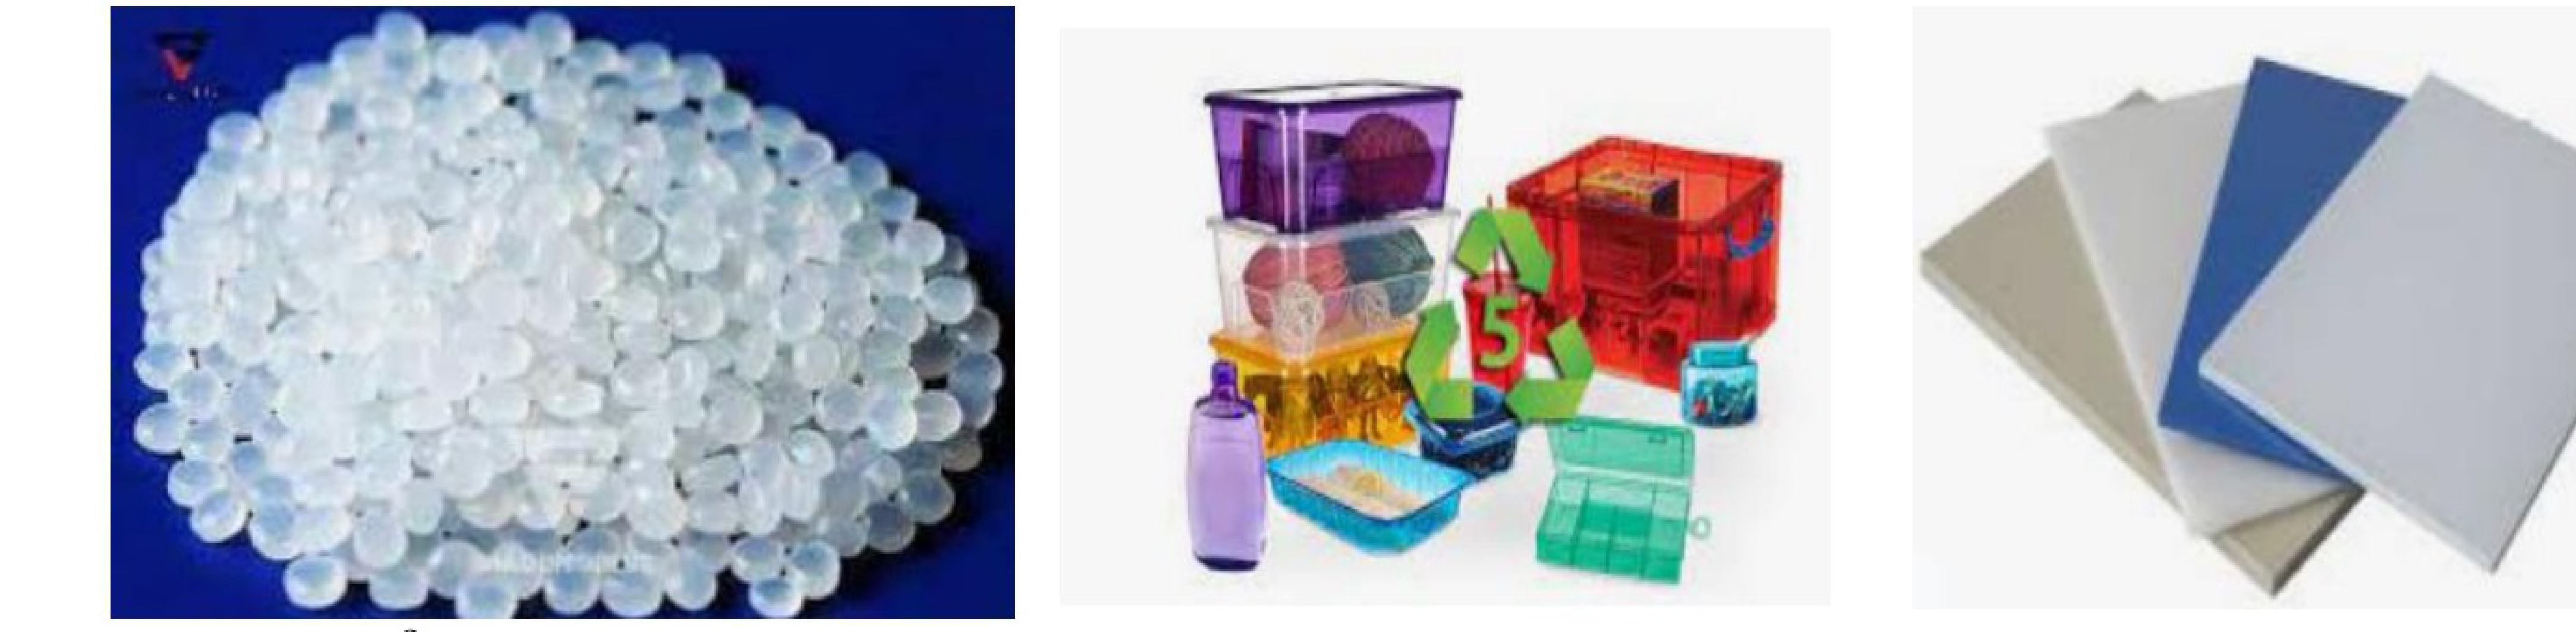
\includegraphics[width=10.5cm]{images_crop_hoa11_de10/hoa11_de10_cau4_pp_products.png}
\end{center}
Phản ứng tạo thành propene từ propyne:
\[\ce{CH3-C#CH(g) + H2(g) ->[t^\circ,\ Pd/PbCO3] CH3-CH=CH2(g)}\]
Từ năng lượng liên kết ($E_b$, kJ/mol) của $\ce{H-H}$ là 432; của $\ce{C-C}$ là 347; của $\ce{C-H}$ là 413; của $\ce{C#C}$ là 839; của $\ce{C=C}$ là 614, hãy tính biến thiên enthalpy chuẩn ($\Delta_r H^\circ_{298}$) của phản ứng tạo thành propene trên theo đơn vị kJ.
\shortans{-169}
\loigiai{
Áp dụng công thức biến thiên enthalpy theo năng lượng liên kết:
\begin{align*}
\Delta_r H^\circ_{298} &= \sum E_b(\text{chất đầu}) - \sum E_b(\text{sản phẩm}) \\
&= [E_b(\ce{C#C}) + E_b(\ce{C-C}) + 4E_b(\ce{C-H}) + E_b(\ce{H-H})] - [E_b(\ce{C=C}) + E_b(\ce{C-C}) + 6E_b(\ce{C-H})] \\
&= [E_b(\ce{C#C}) + E_b(\ce{H-H})] - [E_b(\ce{C=C}) + 2E_b(\ce{C-H})] \\
&= (839 + 432) - (614 + 2 \times 413) \\
&= 1271 - 1440 = -169\text{ kJ}.
\end{align*}
}
\end{ex}

\begin{ex}
(SBT - CTST). Cục Quản Lí Thực Phẩm và Dược Phẩm Hoa Kì (FDA) đã công nhận ethylene là an toàn trong việc kích thích trái cây mau chín. Tuy nhiên khi vượt quá nồng độ cho phép, ví dụ đối với nồng độ 27~000~ppm, tức gấp khoảng 200 lần mức cần thiết để kích thích quá trình chín, một tia lửa điện có thể đốt cháy ethylene và gây ra vụ nổ chết người.\\
Trong phòng ủ chín, ethylene được sử dụng ở nồng độ 100~ppm -- 150~ppm. Khối lượng ethylene cần thiết (tính theo gam, làm tròn đến một chữ số thập phân) sử dụng để phòng ủ chín có thể tích $50\ \text{m}^3$ đạt nồng độ 140~ppm ở $25\ ^\circ\text{C}$ và $1\ \text{bar}$ là bao nhiêu?
\shortans{7{,}9}
\loigiai{
Thể tích phòng ủ: $V_{\text{phòng}} = 50\ \text{m}^3 = 50\ 000\ \text{L}$.\\
Thể tích khí ethylene ở nồng độ $140\ \text{ppm}$ ($1\ \text{ppm} = 10^{-6}$):
\[V_{\ce{C2H4}} = \frac{50\ 000 \times 140}{1\ 000\ 000} = 7\ \text{L}.\]
Số mol ethylene ở điều kiện chuẩn ($25\ ^\circ\text{C}$, 1 bar):
\[n_{\ce{C2H4}} = \frac{7}{24{,}79}\ \text{mol}.\]
Khối lượng ethylene cần thiết:
\[m = \frac{7}{24{,}79} \times 28 \approx 7{,}9\ \text{g}.\]
}
\end{ex}

\begin{ex}
Khí biogas (giả thiết chỉ chứa $\ce{CH4}$) và khí gas (chứa 40\% $\ce{C3H8}$ và 60\% $\ce{C4H10}$ về thể tích) được dùng phổ biến làm nhiên liệu và đun nấu. Nhiệt lượng tỏa ra khi đốt cháy hoàn toàn 1 mol các chất như sau:
\begin{itemize}
    \setlength\itemsep{0pt}
    \item $\ce{CH4}$: 890 kJ
    \item $\ce{C3H8}$: 2220 kJ
    \item $\ce{C4H10}$: 2850 kJ
\end{itemize}
Nếu nhu cầu về năng lượng không đổi, hiệu suất sử dụng các loại nhiên liệu như nhau, khi dùng khí biogas để thay thế khí gas để làm nhiên liệu đốt cháy thì lượng khí $\ce{CO2}$ thải ra môi trường sẽ giảm bao nhiêu phần trăm (làm tròn đến hai chữ số thập phân)?
\shortans{18{,}91\%}
\loigiai{
Gọi $Q$ (kJ) là nhiệt lượng cần cung cấp cho đun nấu.\\
+ Nếu dùng biogas ($\ce{CH4}$):
\[n_{\ce{CH4}} = \frac{Q}{890}\ \text{mol} \implies n_{\ce{CO2}\text{ (biogas)}} = n_{\ce{CH4}} = \frac{Q}{890}\ \text{mol}.\]
+ Nếu dùng khí gas: Tỉ lệ thể tích $\ce{C3H8} : \ce{C4H10} = 40\% : 60\% = 2 : 3$. Đặt $n_{\ce{C3H8}} = 2x\ \text{mol}$ và $n_{\ce{C4H10}} = 3x\ \text{mol}$.
\[Q = 2220 \cdot (2x) + 2850 \cdot (3x) = 12990x \implies x = \frac{Q}{12990}\ \text{mol}.\]
Lượng $\ce{CO2}$ phát thải khi dùng gas:
\[n_{\ce{CO2}\text{ (gas)}} = 3(2x) + 4(3x) = 18x = 18 \cdot \frac{Q}{12990} = \frac{3Q}{2165}\ \text{mol}.\]
+ So sánh lượng phát thải: $\frac{3Q}{2165} \approx \frac{Q}{721{,}67} > \frac{Q}{890}$ nên dùng biogas phát thải ít $\ce{CO2}$ hơn gas.\\
Phần trăm lượng $\ce{CO2}$ giảm đi:
\[\% \text{ giảm} = \frac{\frac{3Q}{2165} - \frac{Q}{890}}{\frac{3Q}{2165}} \times 100\% \approx 18{,}91\%.\]
}
\end{ex}

\vspace{0.3cm}
\noindent\textbf{\large PHẦN IV. Tự luận.}
\textit{Thí sinh trình bày lời giải chi tiết cho các câu hỏi sau.}
\vspace{0.2cm}

\begin{ex}
(1,0 điểm) [CD - SGK]. Cho biết công thức cấu tạo và gọi tên của alkene, alkyne mà khi hydrogen hóa tạo thành butane.

\vspace{4.0cm}

\end{ex}

\begin{ex}
(1,0 điểm). Trong ngành công nghệ lọc hóa dầu, các alkane thường được loại bỏ hydrogen trong các phản ứng dehydro hóa để tạo ra những sản phẩm hydrocarbon không no có nhiều ứng dụng trong công nghiệp:
\begin{center}
    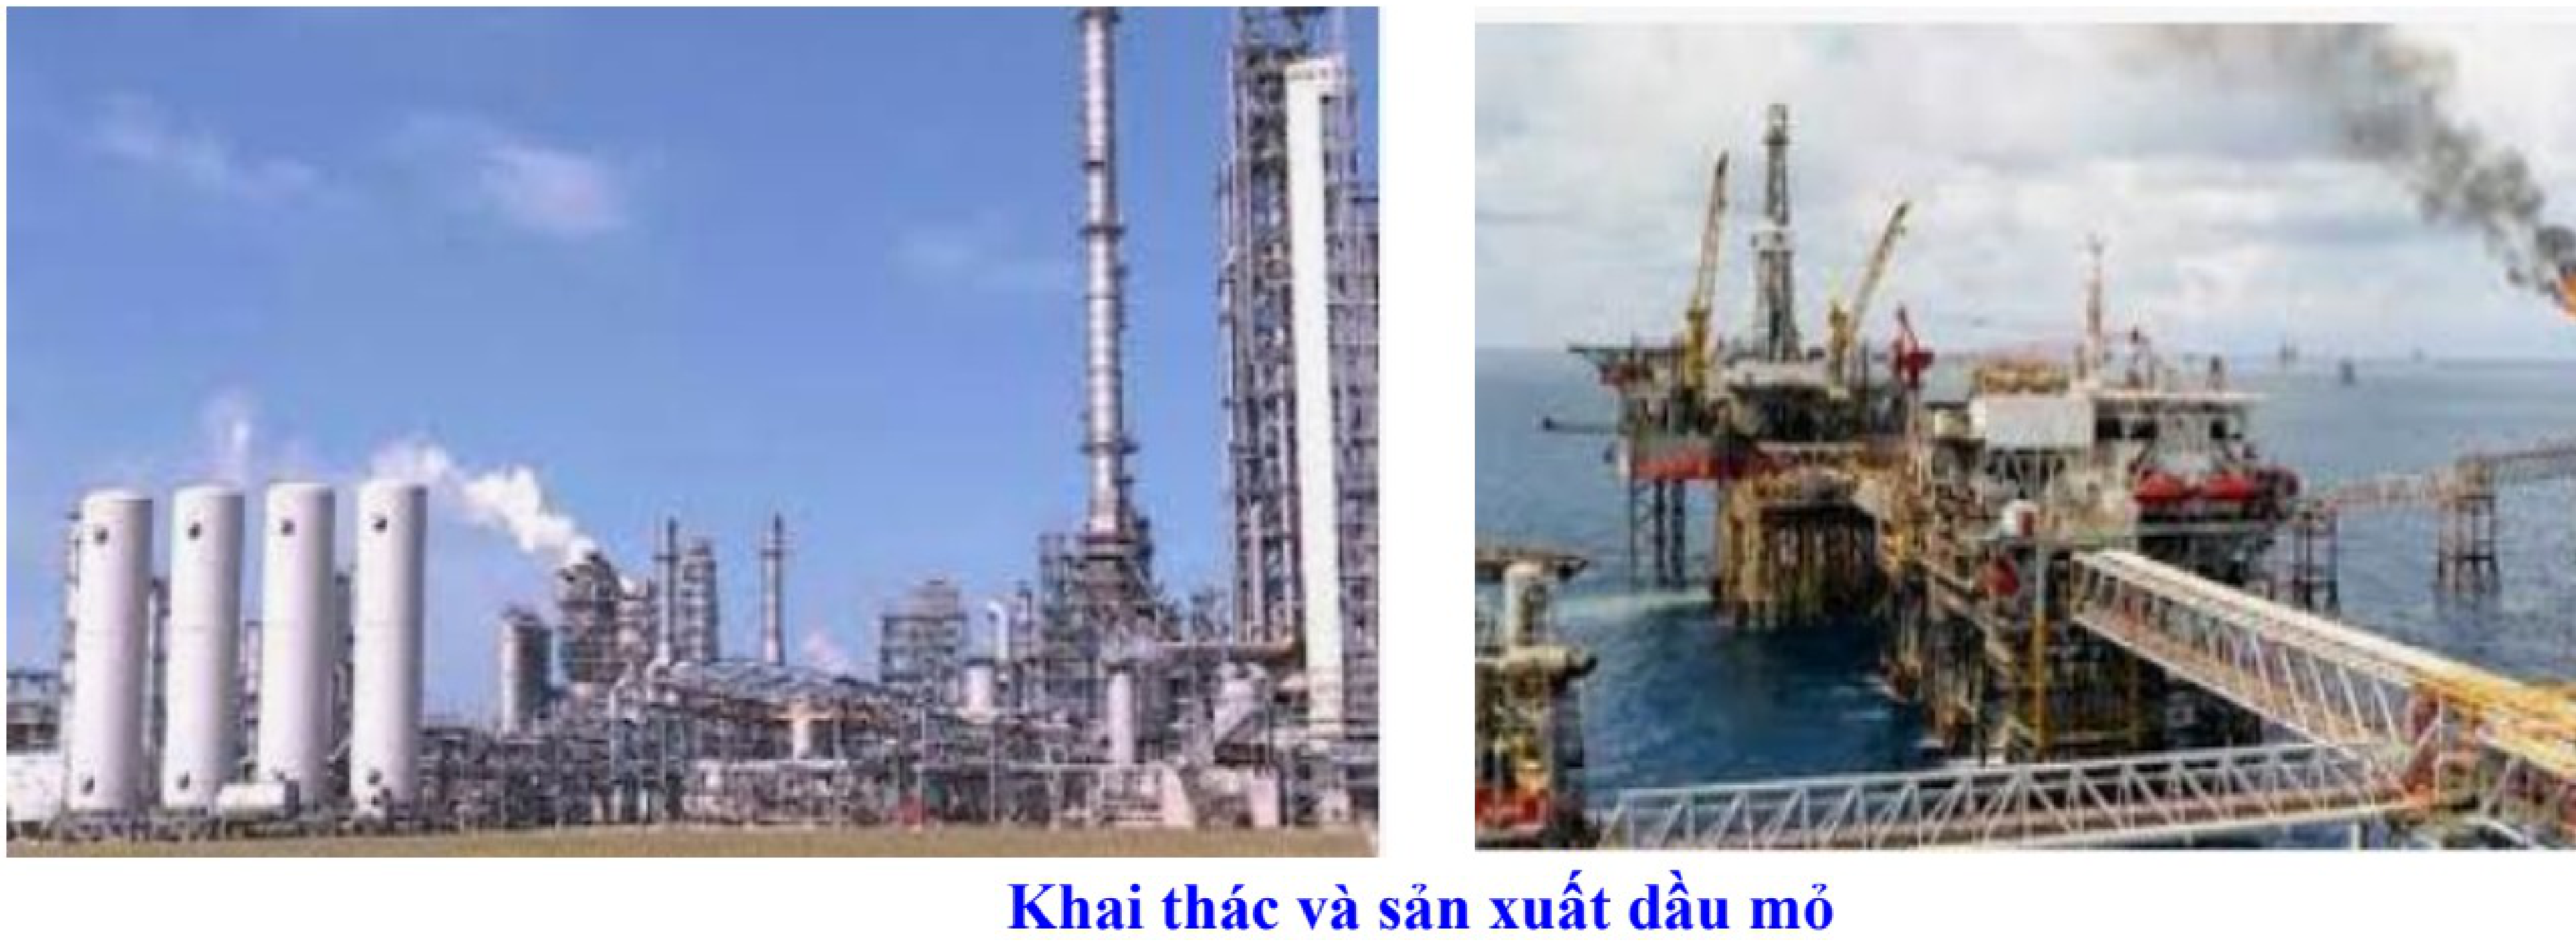
\includegraphics[width=10.5cm]{images_crop_hoa11_de10/hoa11_de10_cau2_oil_refinery.png}
\end{center}
Hãy tính biến thiên enthalpy chuẩn của các phản ứng sau dựa vào năng lượng liên kết:\\
Cho năng lượng liên kết $E_b$ (kJ/mol): $\ce{C-H}$: 414; $\ce{C-C}$: 347 (hoặc 237 theo số liệu đề); $\ce{C=C}$: 611; $\ce{H-H}$: 436.
\begin{enumerate}[a)]
    \item $\ce{H3C-CH2-CH2-CH3 -> CH2=CH-CH=CH2 + 2H2}$
    \item $\ce{6CH4 -> C6H6\text{ (1,3,5-cyclohexatriene)} + 9H2}$
\end{enumerate}
Cho biết công thức cấu tạo của 1,3,5-cyclohexatriene như sau:
\begin{center}
    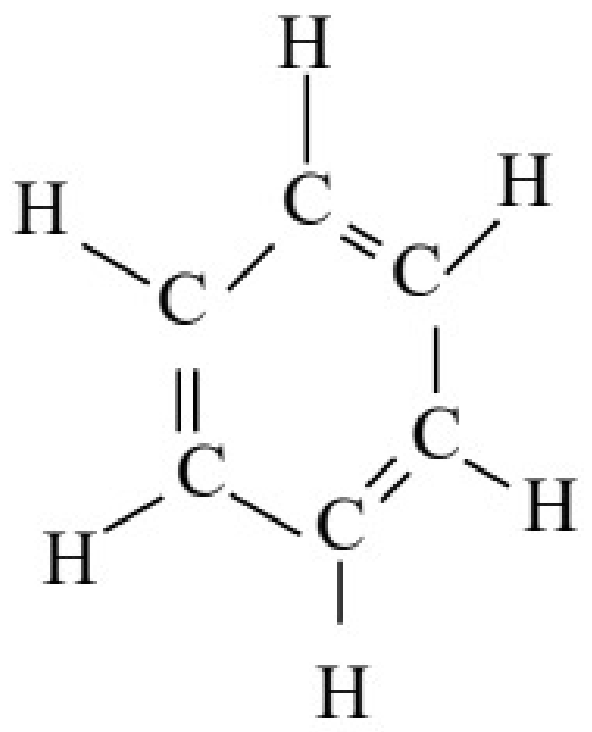
\includegraphics[width=3.2cm]{images_crop_hoa11_de10/hoa11_de10_cau2_cyclohexatriene.png}
\end{center}
Các phản ứng trên có thuận lợi về phương diện nhiệt hay không? Phản ứng theo chiều ngược lại có biến thiên enthalpy bằng bao nhiêu?

\vspace{5.0cm}

\end{ex}

\begin{center}
\textbf{--------- HẾT ---------}
\end{center}

\end{document}
